\section{Paging}

\paragraph{Hierarchical Page Table --- two-level page table}
\begin{itemize}
  \item \textbf{Layout}: on 32-bit machine with 4KiB pages divide virtual address into
  \begin{itemize}
    \item \emph{page number} (p): 20 bits
    \item \emph{page offset} (d): 12 bits
  \end{itemize}
  \item \textbf{Table Paging}: table can be paged to save memory -- subdivide vpn:
  \begin{itemize}
    \item index in \emph{page directory} ($ p_1 $): 10 bits
    \item index in \emph{page table} ($ p_2 $): 10 bits
  \end{itemize}
  \item for ranges of 1024 invalid pages, reset present bit in page directory
  \begin{itemize}
    \item[$ \to $] save space of second-level page table
  \end{itemize}
\end{itemize}
\begin{figure}[h]\centering\label{TwoLevelPageTable}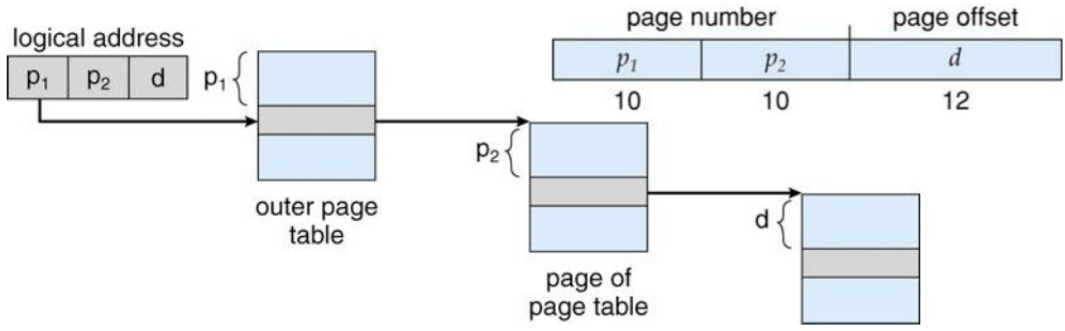
\includegraphics[width=0.33\textwidth]{TwoLevelPageTable}\end{figure}

\paragraph{Linear Inverted Page Table}
\begin{itemize}
  \item \textbf{Problem}: large AS (64 bit) but only few mapped virtual addresses
  \begin{itemize}
    \item[$ \to $] much memory wasted on page tables
    \item[$ \to $] lookup slow due to many levels of hierarchy
  \end{itemize}
  \item \textbf{Idea}: invert page table mapping
  \begin{itemize}
    \item map physical frame to virtual page instead of other way around
    \item single page table for \emph{all processes} (exactly one table per system)
    \item one page table entry for each physical page frame
  \end{itemize}
  \item \textbf{Advantage}: less overhead for page table meta data
  \item \textbf{Disadvantage}: increases time needed to search table when page reference occurs
\end{itemize}
\begin{figure}[h]\centering\label{LinearInvertedPageTable}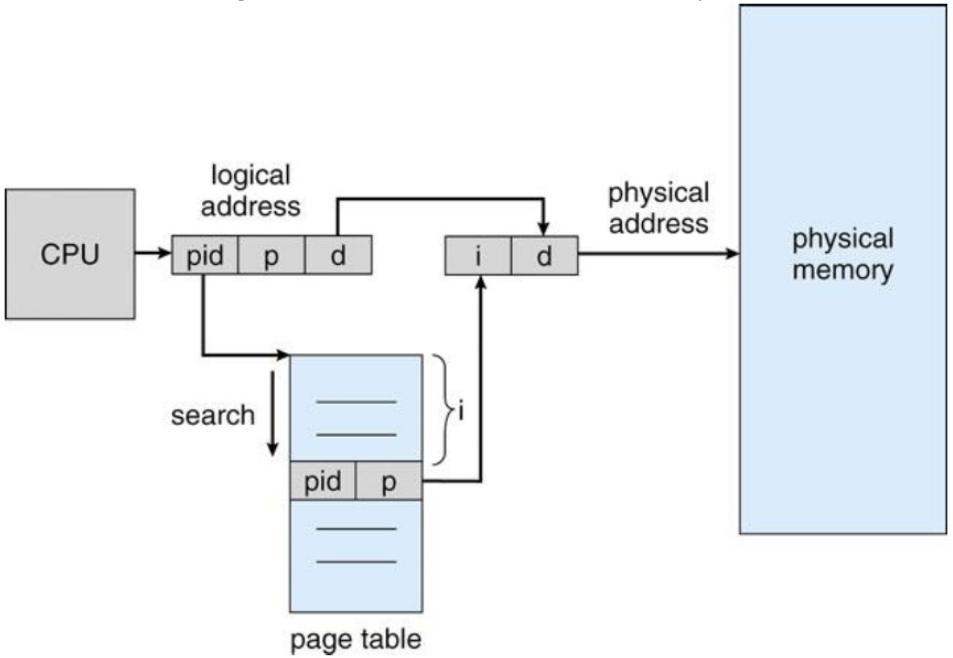
\includegraphics[width=0.33\textwidth]{LinearInvertedPageTable}\end{figure}

\paragraph{Hashed Inverted Page Table}
\begin{itemize}
  \item \textbf{Hash Anchor Table}: limits search to at most a few page-table entries
\end{itemize}

\paragraph{Translation Lookaside Buffer --- Motivation}
\begin{itemize}
  \item \textbf{Naive paging is slow}:
  \begin{itemize}
    \item every load/store requires multiple memory references
    \item 4-level hierarchy: 5 memory references for every load/store (4 page directory/table references, 1 data access)
  \end{itemize}
  \item \textbf{Idea}: add cache that stores recent memory translations
  \begin{itemize}
    \item \emph{translation lookaside buffer} (TLB) maps [vpn] to [pfn, protection]
    \item typically 4-way to fully associative hardware cache in MMU
    \item typically 64-2048 entries
    \item typically 95\%-99\% hit rate
  \end{itemize}
\end{itemize}

\paragraph{TLB --- Operation}
\begin{itemize}
  \item on every load/store:
  \begin{itemize}
    \item check if translation result is cached in TLB (\emph{TLB hit})
    \item otherwise walk page tables, insert result into TLB (\emph{TLB miss})
  \end{itemize}
  \item \textbf{Quick}: can compare many TLB entries in parallel in hardware
\end{itemize}

\paragraph{TLB --- TLB Miss}
\begin{itemize}
  \item \textbf{Process}:
  \begin{itemize}
    \item evict entry from TLB on TLB miss
    \item load entry for missing virtual address into TLB
  \end{itemize}
  \item \textbf{Variants}: \emph{software-managed} and \emph{hardware managed}
  \item \textbf{software-managed TLB}:
  \begin{itemize}
    \item OS receives \emph{TLB miss exception}
    \item OS decides which entry to evict (drop) from TLB
    \item OS generally walks page tables in software to fill new TLB entry
    \item TLB entry format specified in \emph{instruction set architecture} (ISA)
  \end{itemize}
  \item \textbf{hardware-managed TLB}:
  \begin{itemize}
    \item evict TLB entry based on hardware-encoded policy
    \item walk page table in hardware $ \to $ resolve address mapping
  \end{itemize}
\end{itemize}

\paragraph{TLB --- Address Space Identifiers}
\begin{itemize}
  \item \textbf{Problem}: vpn dependent on AS
  \begin{itemize}
    \item vpns in different AS can map to different pfns
    \item[$ \to $] need to clear TLB on AS switch
  \end{itemize}
  \item \textbf{Idea}: solve vpn ambiguity with additional identifiers in TLB
  \item \textbf{ASID}: TLB has \emph{address space identifier} (ASID) in every entry
  \begin{itemize}
    \item map [vpn, ASID] to [pfn, protection]
    \item[$ \to $] avoids TLB flush at every address-space switch
    \item[$ \to $] less TLB misses: some TLB entries still present from last time process ran
  \end{itemize}
\end{itemize}

\paragraph{TLB --- Reach}
\begin{itemize}
  \item[=] amount of memory accessible with TLB hits: $ \text{TLB reach} = \text{TLB size} * \text{page size} $
  \item \textbf{Ideally}: working set of each process is stored in TLB (otherwise high degree of TLB misses)
  \item \textbf{Increase page size}:
  \begin{itemize}
    \item[+] fewer TLB entries per memory needed
    \item[-] increase internal fragmentation
  \end{itemize}
  \item \textbf{multiple page sizes}:
  \begin{itemize}
    \item[+] allows applications that map larger memory areas to increase TLB coverage with minimal fragmentation increase
  \end{itemize}
  \item \textbf{increase TLB size}:
  \begin{itemize}
    \item[-] expensive
  \end{itemize}
\end{itemize}

\paragraph{TLB --- Effective Access Time}
\begin{itemize}
  \item \textbf{Associative lookup}: takes $ \tau $ time units (e.g., $ \tau = 1\text{ns} $)
  \item \textbf{Memory cycle}: takes $ \mu $ time units (e.g., $ \mu = 100\text{ns} $)
  \item \textbf{TLB hit ratio} $ \alpha $: percentage of all memory accesses with cached translation (e.g., $ \alpha = 99\% $)
  \item \textbf{Effective Access Time} (EAT) for linear page table without cache:
    \begin{equation*}
      \text{EAT} = (\tau + \mu)\alpha + (\tau + 2\mu)(1-\alpha) = \tau + 2\mu - \mu\alpha
    \end{equation*}
\end{itemize}

\begin{summary}
  \begin{itemize}
    \item page tables communicate between OS and MMU hardware
    \begin{itemize}
      \item how virtual addresses in each address space translate to physical addresses
      \item which kind of accesses the MMU should allow/signal to the OS
    \end{itemize}
    \item different page table layouts have been developed
    \begin{itemize}
      \item linear page table
      \item hierarchical page tables
      \item inverted page tables
      \item hashed page tables
    \end{itemize}
    \item performing page table lookups for every memory access significantly slows down execution time of programs
    \begin{itemize}
      \item translation lookaside buffer (TLB) caches previously performed page table lookups
      \item typical TLBs cover $ 95\%-99\% $ of all translations
    \end{itemize}
  \end{itemize}
\end{summary}
